\section{Populating Tables With Data}

Now that we have successfully created all the necessary data, it is time to fill them with data. We will use a variety of different methods to import data to our tables.

\subsection{Populating Users}

We retrieved a large excel file containing over one hundred thousand users' data from the internet, but since we had no remaining space in the database we had to shrink that file to only one thousand records. Using the PL/SQL Developer tool called ODBC importer we imported the data which we needed into the users table. Not all of the columns provided were necessary to us, so figure \ref{users-odbc} shows which columns we used. The excel file which we used can be found in \verb`/data/users/user_list.xlsx`.

\begin{figure}[hbtp]
	\centering
	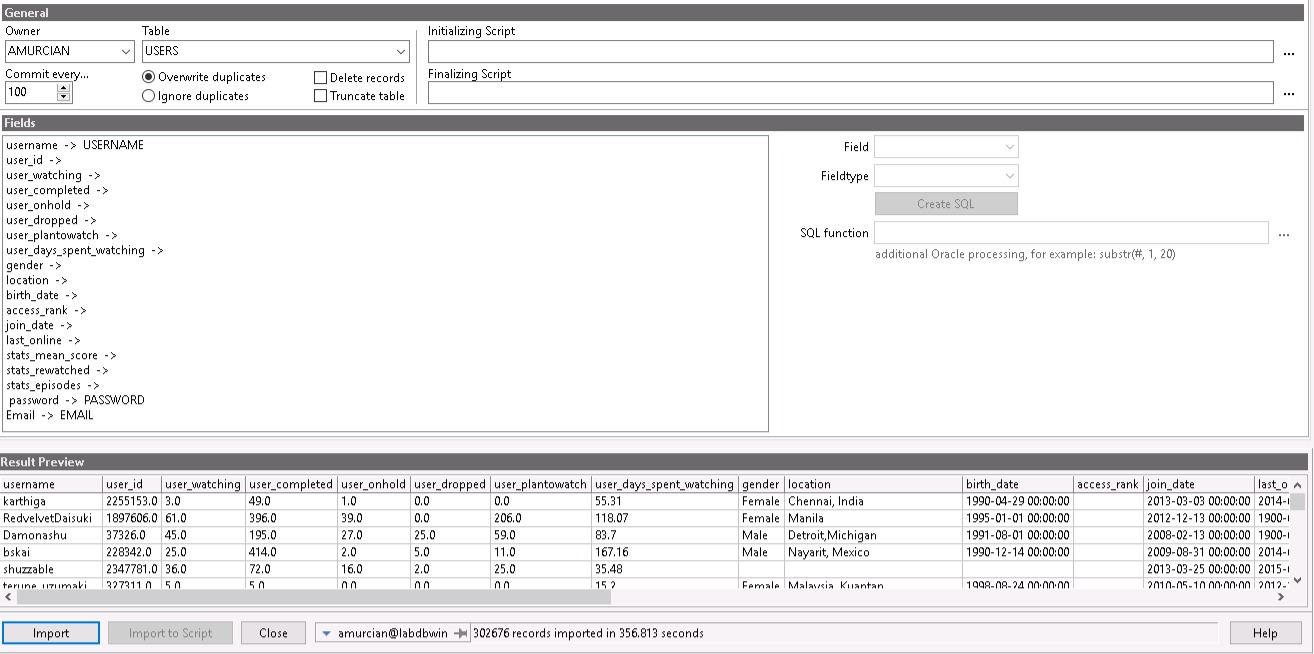
\includegraphics[width=\linewidth]{images/users_odbc.jpeg}
	\caption{A screenshot showing how the ODBC importer imported our data}
	\label{users-odbc}
\end{figure}

\subsection{Populating Posts}

Since this table only contains one column, and that column's value was always generated by the database, this simple script was enough to insert the required number of post IDs into the post table. We originally had inserted over 200,000 but due to severe space constraints we reduced this to 3,000.

\VerbatimInput[label=\fbox{\color{Black}/sql/insert/posts.sql}]{../../sql/insert/posts.sql}

\subsection{Populating Questions}

We were able to obtain a CSV file containing all of the questions which were asked on \LaTeX\ Stack Exchange between January 2010 and September 2020. Since we were restricted on space, we manipulated the CSV file using spreadsheet software to keep only the 1,000 shortest questions. After appending an ID from those which we inserted into the \verb`posts` table to each row, and removing all columns which we do not need, we ran the text importer tool in PL/SQL Developer to add all of the data in the CSV file into the \verb`questions` table.

Figure \ref{questions-text-import} shows the configurations for the text importer which was used to import the questions from our CSV file.

\begin{figure}[htbp]
	\centering
	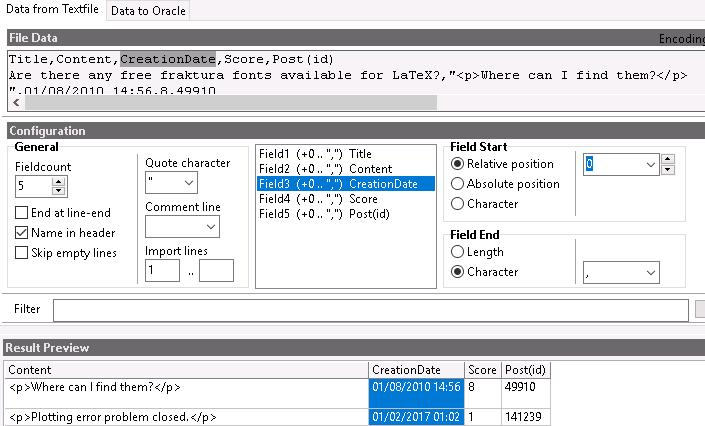
\includegraphics[width=\linewidth]{images/questions_text_import_1.jpeg}
	\vspace{2em}
	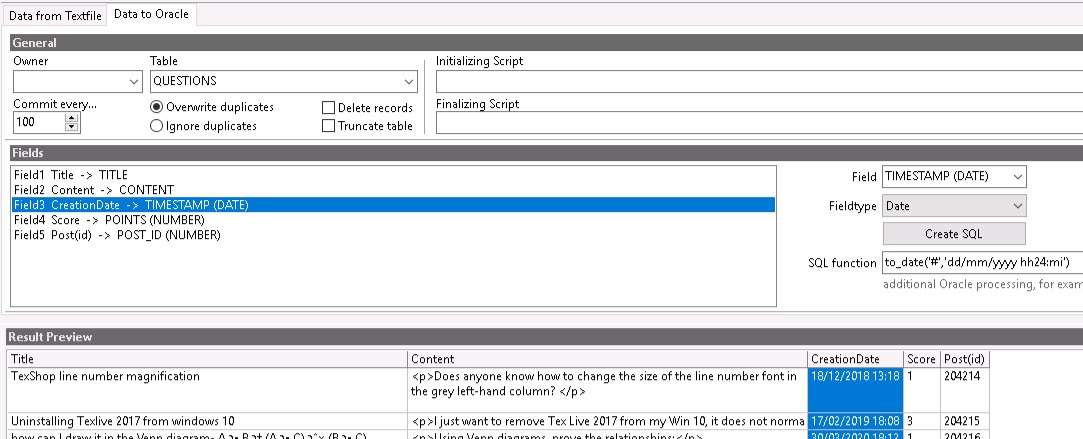
\includegraphics[width=\linewidth]{images/questions_text_import_2.jpeg}
	\caption{The configurations in the text importer for the questions table}
	\label{questions-text-import}
\end{figure}

\subsection{Populating Answers}

We used the data generator tool in PL/SQL developer, as shown in figure \ref{answers-generator}, to populate this table with 1,000 random records.

\begin{figure}[htbp]
	\centering
	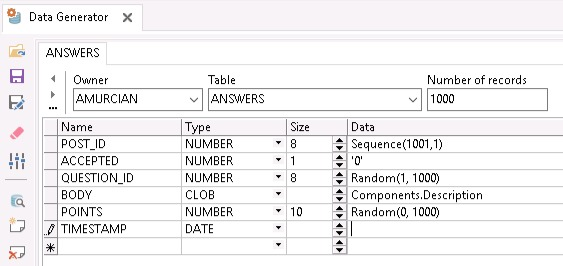
\includegraphics[width=\linewidth]{images/answers_generator.jpeg}
	\caption{The configurations in the data generator tool for the answers table}
	\label{answers-generator}
\end{figure}

\subsection{Populating Comments}

We used the data generator tool to generate 1,000 random comments, but in order to avoid randomly generating circular ancestry with comments, we assigned all comments to a single question. Then we exported the data as a CSV which we then modified so that each comment referenced a post with an ID smaller that the ID of that comment. We then truncated the table to remove the random data, and used the text importer to import the processed CSV in the same way which we imported the questions. This CSV file can be found at \verb`/data/comments/comments.csv`

\subsection{Populating Topics}

We were able to find a large list with 1,547 topics which Quora uses to organise their questions. We obtained it in the form of a plain text file with one line for each topic name. Since it contains duplicates, we can must first remove these. Then we generate some randomised description using the python module called \verb`lorem`. This python code shows exactly how the insert statements were generated. The generated SQL code can be found at \verb`/sql/insert/topics.sql`

\VerbatimInput[label=\fbox{\color{Black}/data/topics/topics\_to\_insert.py}]{../../data/topics/topics_to_insert.py}

\subsection{Populating Votes}

We used the data generator to populate this table. The settings we used to generate the random data is practically identical to those seen in figure \ref{follows-generator}.

\subsection{Populating Follows}

This table was populated using the data generator tool in PL/SQL Developer. We asked the system to generate a number from the users' ID column for the foreign key to that row, and similarly for the other foreign key. Figure \ref{follows-generator} shows the settings we used to generate 1,000 rows.

\begin{figure}[htbp]
	\centering
	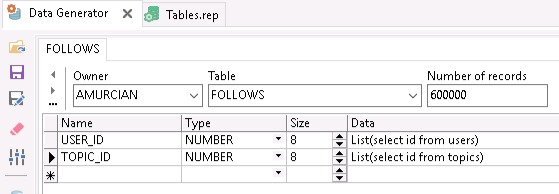
\includegraphics[width=\linewidth]{images/follows_generator.jpeg}
	\caption{Settings used for generating the follows table data}
	\label{follows-generator}
\end{figure}

\subsection{Populating Relates To}

This table also had its data generated in the same way as the \verb`follows` and \verb`relates_to` tables.